\chapter{Hierarchy of Networks}
\label{cha:HierarchyOfNetworks}
\markright{Hierarchy of Networks}

\section{Introduction to Network Hierarchy}
Hierarchy is a method used in creating scalable and complex systems. It is based on abstraction, at each level, of the most significant of details to the levels further away. Specifically in communication networks, hierarchy is an abstraction of parts of the network's topology, routing or signaling mechanisms. Here, abstraction or aggregation of information is used as a technique to achieve scalability in large networks, or for enforcing administrative, topological, or geographic boundaries. For example, network hierarchy might be used to separate the metropolitan and long-haul regions of a network, to separate the regional and backbone sections of a network, or to interconnect service provider networks.

In our study, we will concentrate on the network hierarchy from two perspectives: 

\begin{enumerate}
\item \emph{Vertical hierarchy}: between two network technology layers. 
\item \emph{Horizontal hierarchy}: between two areas or administrative subdivisions within the same network technology layer.
\end{enumerate}


\subsection{Multilayer Horizontal Network Hierarchy}

\begin{figure}[ht]
 \centering 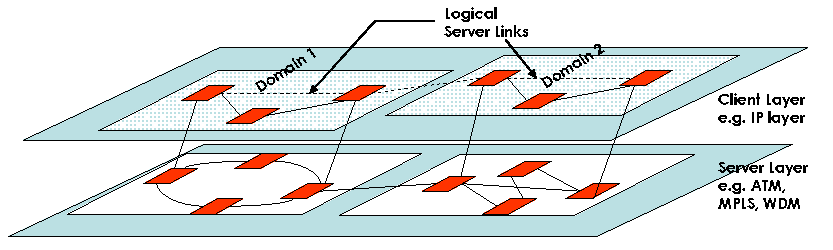
\includegraphics{Figures/HorizLayers} 
\caption{Horizontal hierarchy separation in transport networks}
\label{fig:HorizLayers} 
\end{figure}

Multi-domain horizontal hierarchy is the abstraction that allows a network to scale at certain technology layer, for instance a packet network. Examples of horizontal hierarchy include BGP confederations, separate Autonomous Systems (\gls{AS})s, and multi-OSPF areas.

In the horizontal hierarchy, a large network is partitioned into multiple smaller, non-overlapping sub-networks. The partitioning criteria can be based on topology, network function, administrative policy, or service domain demarcation. Two networks at the same hierarchical level, e.g., two ASes in BGP, may share a peer relation with each other through some loose form of coupling. On the other hand, for routing in large networks using multi-area OSPF, abstraction through the aggregation of routing information is achieved through a hierarchical partitioning of the network.

\subsection{Multilayer Vertical Network Hierarchy}
In multilayer vertical hierarchy, the total network functions are partitioned into a series of functional or technological layers with clear logical, and sometimes physical separation between adjacent layers. Vertical hierarchy, hence, is a generalization that reduces the communication overhead when propagating information across various switching layers of the network; for example, when propagating information between optical and packet switching layers. Figure~\ref{fig:ClientServerLayers} shows interactions between adjacent vertical layers of a network element, as well how vertical network layers form adjacencies between adjacent peering network elements.

\begin{figure}[ht]
 \centering 
 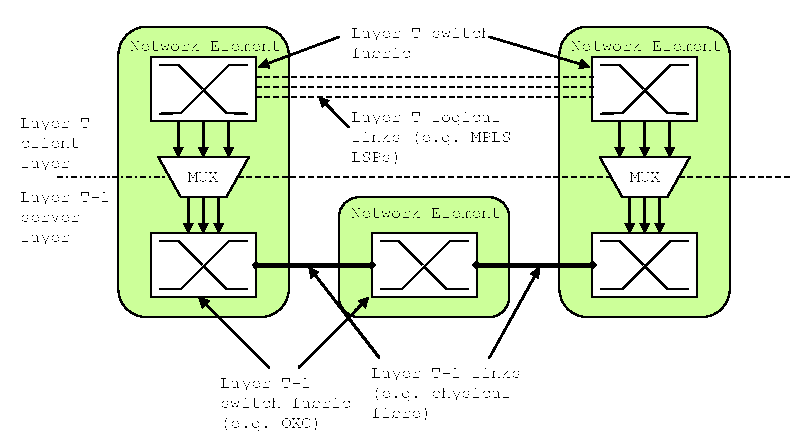
\includegraphics{Figures/ClientServerLayers} 
 \caption{Client-server relationship between vertical layers of network hierarchy.}
\label{fig:ClientServerLayers} 
\end{figure}

\section{GMPLS and Hierarchical Networks}
Several architectural models for the control plane of multilayered networks are in existence today, including the overlay, augmented or border, and the peer models. One of the key differences among these models is how much, and what kind of network information is exchanged between individual layers. \emph{Vertical integration} refers to the collaborative mechanisms within a single control plane instance driving multiple (but at least two) data planes (also referred to as switching layers). \emph{Horizontal integration}, on the other hand, refers to the collaborative mechanisms of control planes extending over several partitions (e.g. IGP areas or autonomous systems) within the scope of at least one data plane instance or veridical switching layer. In this case, the relation between the various horizontal partitions constitutes a peer-to-peer relationship as opposed to a client-server relationship as in the case of vertical integration model {[}KOO04].

\subsection{Overlay Model}
In the overlay network model, the nodes in each layer maintain network information about nodes and links residing in the same layer- such as residual capacity on existing logical links and number of available ports- which makes it more suitable in the case with different management/ownership in each layer. The upper layer only receives a response from the adjacent lower layer on whether or not the requested connection can be set up. There is no specific network information exchanged between individual layers, since the routing in each layer is done separately with each layer's own signaling and control plane.

Hence, in this model, each network layer has to decide whether it will use the existing logical links in its topology or try to create new connections/logical links, and how to route the new request over the existing logical topology without any network information from the lower layer. Each layer's control plane is strictly separate from its adjacent one and runs its own routing and signaling instance protocols,and no information is shared among the two.

\subsection{Peer Model}
In the peer model, the topology and other network information (\eg routing and link state) are shared among all network elements across all the layers by a unified signaling protocol and control plane (\eg single control plane instance for packet and optical layers). Such a model is appropriate when the transport and service networks are operated by a single entity.

In this model, each LSR keeps information about the topology and status of links (\eg bandwidth availability on packet links, and availability of each wavelength at the WDM layer) as well as logical links in the IP/MPLS layer. As often visualized, a network in the peer model can be seen as one graph with both LSRs and OXCs interconnected with physical and logical edges. In this case, an integrated routing can be done with a unified control plane. For example, the integrated routing scheme decides routing over existing logical links, and routing and wavelength assignment (RWA) in the WDM layer at the same time. Note that this is a fundamental difference in the dynamic \gls{LSP} provisioning problem between the peer model and the other two models. In the overlay and augmented models, the RWA in the WDM layer is beyondthe scope of the \gls{LSP} provisioning problem in the IP/MPLS layer.

While in the overlay model global resource usage optimization is not guaranteed - since every layer is optimized in isolation, in the peer model, all layers collaborate in order to achieve some common performance objectives. In this case, a globally optimum solution does not necessarily mean that the individual layers are also optimized. In the peer model, each network node has complete knowledge about the network status (traffic flows, links used, available optical resources, and available capacity in the already established routes), and the entire network can self-adapt dynamically to traffic changes.

\subsection{Border Model}
The border model (also known as the augmented model) provides a compromise between the two extreme cases of peer and overlay models by running separate routing protocols in each layer but still allowing the exchange of partial network information between them- for example, reachability and/or summary of link state information and residual capacity -- depending on a necessary and specific agreement between the two layers.

For example, the IP/MPLS switching layer may utilize a small amount of capacity information passed from the WDM switching layer- for example, the number of lightpaths that the WDM layer can further provide between
every LSR pair in the current state of the WDM network. Hence, a network in the augmented model has to make the same provisioning decision as in the overlay model except that it has more information about the status of the adjacent layers.

\section{Quality of Service}
The notion of \gls{QoS} and network performance are defined in ITU-T Recommendation E.800 (ITU94) as follows:

\begin{quotation}
\emph{{}``The Quality-of-Service is the collective effect of service performances that determine the degree of satisfaction of a user of the service. The Network performance is the ability of a network portion to provide the functions related to communications between users.''} 
\end{quotation}

End-to-end \gls{QoS} ordains that all network layers from top-to-bottom, as well as every network element from end-to-end work collaboratively to provide the desired level of \gls{QoS}. Any \gls{QoS} assurances are only as good as the weakest link in the chain between sender and receiver. End-to-end \gls{QoS} service can be achieved by signaling and reserving the network resources in advance before transferring data.

Often, \gls{QoS} is seen as the need for networks to provide performance bounds on offered services. In other instances, \gls{QoS} is measured in terms of network survivability or availability in the presence of failures. The traditional best-effort Internet was not designed to support a specified, desired, or consistent level of \gls{QoS} to network traffic. Nonetheless, customers now require mission critical services-- such as corporate \gls{VPN}s and radio access networks that demand high levels of network availability and guaranteed levels of service under heavy traffic loads. Service providers now use sophisticated \gls{TE} mechanisms to manage their networks to meet these demands.

\subsection{QoS in Multilayered Networks}
As mentioned, \gls{SLA} levels and \gls{QoS} parameters can be defined on all seven levels of the OSI network model. For example, the Differentiated Services (\gls{Diffserv}) defines mechanisms to provide service differentiation at layer-3 IP packets. At the \gls{MPLS} layer other models, e.g. EXP-inferred \gls{LSP}s (E-\gls{LSP}s) and label inferred \gls{LSP}s (L-\gls{LSP}s), are used to ensure \gls{QoS} for \gls{MPLS} traffic. At switching layer 2, Ethernet's 802.1p and ATM classes of service (CoS) are used to assure \gls{QoS} to traffic traversing at these layers. At layer 1 (WDM layer), \gls{QoS}
is provisioned by introducing schemes to partition wavelengths and classify them into different sets, each being used to service one or more traffic types. This segregation prevents traffic of one type impacting another. \gls{MPLS} preemption based on \gls{LSP} priority is another feature that provides a way to define the relative importance of \gls{LSP}s that compete for the available resources; for example, it allows the preemption of low-priority \gls{LSP}s in favor of higher-priority \gls{LSP}s within a single switching layer. Moreover several service policies can exist for the definition of \gls{LSP} priorities between different layers.

It is imperative, therefore, that \gls{QoS} parameters at all layers of the communication network be considered in the calculation of a potential path for assuring end-to-end \gls{QoS}. A multilayer \gls{QoS} routing system will require performing the following tasks: 2) aggregate \gls{QoS} information to other levels of the network hierarchy, 1) disseminate \gls{QoS} information parameters, and 3) provide the exact hierarchical \gls{QoS} path computation and resource reservation schemes.

\begin{figure}
 \centering 
 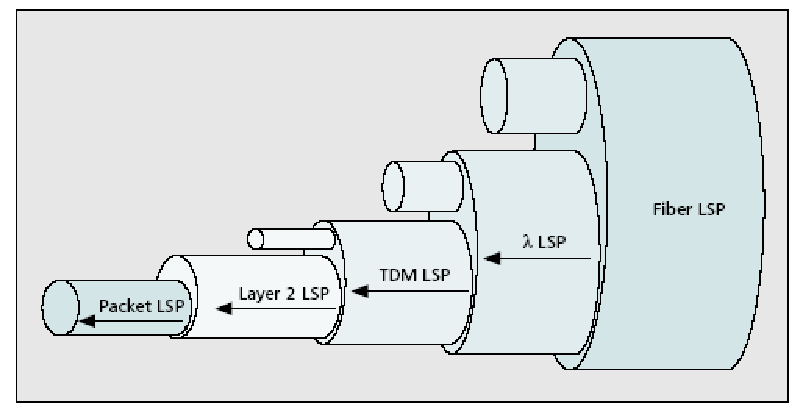
\includegraphics[scale=1]{Figures/HierarchicalLsps}
 \caption{LSP hierarchy in multilayered GMPLS networks}
\label{fig:HierarchicalLsps}
\end{figure}

\subsection{QoS and Traffic Engineering in Multilayered Networks}
The main objective of Traffic Engineering (\gls{TE}) is to improve the efficiency and reliability of networks while optimizing resource utilization and traffic performance. \gls{TE} solutions enable the fulfillment of all these requirements by allowing the network to choose routes for traffic flows while taking into account the amount of traffic load and the network state, or to react to rapid traffic changes or network failures in short time intervals. These solutions can be adopted by using an intelligent unified control plane (such as \gls{GMPLS}), which is able to adequately handle network resources.

Traffic engineering and QoS are strongly related, but to make a difference, QoS controls how the resources are allocated to different users, whereas TE controls where in the network resources are used. Performance optimization of IP networks can be done both at the traffic level and at the resource level. Traffic oriented performance concentrates on the quality of service of traffic streams. Minimization of packet loss and delay, maximization of throughput and execution of service level agreements are the major measures to be improved. The resource oriented performance objectives consist of efficient resource utilization and resource management. Usually bandwidth is the most scarce resource, so a major function is to manage bandwidth allocation.

Both from traffic and resource oriented perspectives the minimization of congestion is crucial. Congestion can be divided into two types, congestion in the case
where resources are insufficient to carry all the traffic, and congestion in the case where resources are divided inefficiently so that a part of network is over-utilized while another part of network has unused bandwidth. The second type of congestion is usually the topic of studies that attempt to minimize it by using techniques provided by traffic engineering by minimizing the maximum TE link utilization. However, TE should still be carried out in such a way that congestion can be managed cost-effectively. 

Performance optimization of networks is actually a control problem. Traffic engineering should provide sufficient control in an adaptive feedback control system. The tasks of a controller consist of modification of traffic management parameters, modification of routing parameters and modifications of resource attributes and constraints [RFC2702].

MPLS-\gls{TE} in packet-based networks provides efficient bandwidth utilization by rerouting traffic via links that are under-utilized. Extensions were defined to enable hierarchical \gls{LSP} establishment-- \eg packet over optical \gls{LSP}s for hierarchical \gls{LSP}s nested inside existing higher-order LSPs. In this case, the preexisting lower-order \gls{LSP} serves as a link along the path of the new \gls{LSP}. Devices form different regions based on their multiplexing capabilities. For example, photonic cross connects define Fiber Switching Capable (\gls{FSC}) devices, Optical Cross Connects (\gls{OXC}s) define the Lambda Switching Capable (\gls{LSC}) devices, L2 switched define the layer-2-switching-capable devices, SONET cross connects define the time division multiplexing (\gls{TDM}) devices, and routers/LSRs define the Packet Switching Capable (\gls{PSC}) nodes. \gls{LSP}s that start and end in a \gls{PSC} region can be combined and nested into an LSP of type \gls{TDM}. \gls{TDM} LSPs in turns can be nested inside an LSC type LSP which can be nested into an FSC type LSP-- as shown in Figure~\ref{fig:HierarchicalLsps}. The new LSPs can be flooded into the routing database to appear as a TE Links.

To perform path computation, a node is able to use conventional links as well as existing LSPs. In optical networks, the traffic coming from upper layers such as IP, ATM, MPLS or SONET/SDH is carried over the logical topology defined by the set of established lightpaths. TE solutions address routing schemes for lightpath set-up, intelligent reconfiguration of the virtual network connectivity (topology), as well as to protection or restoration schemes for lightpath recovery. In a 2-layer IP over \gls{WDM} model, TE can be performed in two main methods, depending on the knowledge of the traffic demand and the level of integration between layers (e.g. overlay, full-peer, or border model).

If traffic demand is known only in terms of an aggregated traffic matrix, the problem of automatically updating the configuration of an optical network to accommodate traffic changes is referred to as Virtual Topology Reconfiguration (VTR). If instead the traffic demand is known in terms of data-level connection requests with sub-wavelength granularity, arriving dynamically from some source node to any destination node, the problem is called Dynamic Traffic Grooming (DTG).

The Traffic Grooming problem has been proven to be NP-hard; thus, heuristics that provide sub-optimal solution are usually applied when connection requests arrive dynamically in realtime. Although many algorithms have been developed to deal with this problem, little attention has been put so far on the \gls{QoS} guarantees for the traffic that simultaneously spanns vertical as well as horizontal layers of
the network hierarchy.

\section{VPNs in Multilayered Networks}
Today, there is increased interest from service providers in offering diverse services and transport solutions for different traffic types over a single common infrastructure. A Virtual Private Network (\gls{VPN}) is usually defined as an overlay network that is built over a public network infrastructure, providing its users with a private and secure network using tunneling, encryption, as well as authentication mechanisms {[}KHA04]. \gls{VPN}s are usually built over various types of public provider networks, such as Frame Relay, ATM or the Internet. \gls{VPN}s are technically classified based on two factors: 1) the underlying technology stack of the backbone transport network that carries the \gls{VPN} application�s traffic (\eg Layer-3 IP/MPLS, Layer-2 SONET/SDH and ATM, or Layer-1 \gls{WDM} core switching networks), or 2) the tunneling endpoint switching layer (\eg Layer-2 Ethernet, Frame Relay or ATM tunnels, or Layer-3 IP tunnels). Figure~\ref{fig:VPNSchemes} shows several \gls{VPN} models that have been proposed to date. For example, a Layer-3 VPN forwards packets based on the \gls{VPN} customer�s IP information, while a Layer-2 \gls{VPN} forwards Layer-2 frames based on information in custaomer's VLANs, MAC addresses, ATM VC Connection Identifiers (VCID), etc. Both of the previous mentioned examples, however, can be carried over a Layer-1, Layer-2, or Layer-3 core based network. Two major flavors of VPNs exist: Provider Edge based (PE-based) and the Customer Edge based (CE-based). Both offer transport services for Layer-2 as well as Layer-3 traffic.

\begin{figure}[ht]
 \centering 
 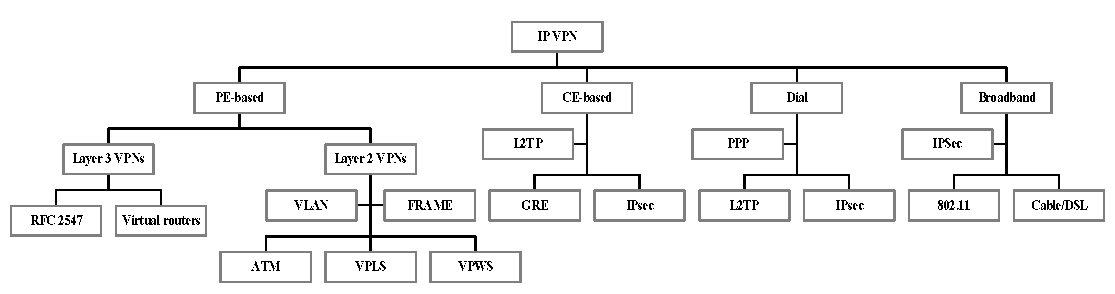
\includegraphics[scale=0.85]{Figures/VPNSchemes}
 \caption{IP VPN protocol implementation schemes.}
\label{fig:VPNSchemes} 
\end{figure}


\subsection{VPN Security}
Security is considered a key aspect in implementing VPNs. To achieve maximum security, customers� encryption and authentication are usually required. Encrypting the customer�s \gls{VPN} traffic prevents other customers in other VPNs from sniffing the data in case of misrouting within the provider�s network. Moreover, authenticating customer \gls{VPN} traffic filters incoming traffic at the Customer Edge or Provider Edge to ensure authenticity of the received traffic. As shown in Figure 1, there are two basic security models that exist within \gls{VPN} implementations: 1) Provider-Edge based security model and 2) the Customer-Edge based security model. In the PE-based model the provider manages and secures communication of traffic crossing its edge boundaries, whereas PE-CE links fall out of its scope of responsibility. In the CE-based \gls{VPN} security model, the connection�s security is covered from end-to-end. The security rules and configuration are done at the customer's side and the provider's edge only provides a transparent media for end-to-end connectivity. Hence, the CE-based security model inherently provides a more stringent and secure implementation of \gls{VPN} than its PE-based counterpart. MPLS and \gls{VLAN}s, by themselves, provide little security for traffic transported over them. In order to enhance security, it is possible to augment them with IP sec tunnels that run from PE-to-PE. This consists of applying IPsec in transport mode to IP tunnels transported over tagged \gls{VLAN}s or MPLS LSPs. The \gls{VLAN} tags or MPLS labels are used ensure privacy and segregate traffic from different VPNs.

Within the Service Provider network, forwarding is based on labels, not on IP addresses carried in the packets. The MPLS switching paths for \gls{VPN} traffic originate and terminate at a PE. They do not begin or terminate in the middle of the Service Provider network. Logical ports on the PEs are associated with VRFs and thus with VPNs at the provisioning time.

MPLS \gls{VPN} privacy is similar to the traditional form of WAN such as Frame Relay and ATM. It provides separation of the traffic between the private customers' networks carried on the Service Provider backbone. MPLS \gls{VPN} establishes network privacy via constrained distribution of routing information and encapsulation of the \gls{VPN} site traffic with a label header in order to traverse an MPLS core. It does not, however, provide firewall security or encryption on the packet, so when \gls{VPN} sites are connected to Extranets or the Internet, additional security measures are necessary to maintain the customer network privacy.

\subsection{VPN Reliability}
Existing transport networks run a variety of network technology layers such as IP, ATM, Gigabit Ethernet, SONET, and \gls{DWDM}. The degree of availability of a connection depends on the proper identification and selection of the protection layer through which the connection traverses. In general, a connection can be protected against failures that occur at the uppermost containing layer as well as layers that fall below. For instance, in a traditional IP multi-layered transport network, a protection layer for a connection can be any of the layers IP, ATM, SONET, down to DWDM. It is possible to apply redundancy or protection techniques at one or more of the transport network layers. However, care should be taken to the tradeoffs between recovery-time and network resource utilization when choosing the appropriate protection  layer. There are mainly two methods for implementing protection on any of these layers: 1) the proactive approach-- typically referred to as protection, and 2) a reactive approach-- also referred to as restoration. In the proactive approach spare capacity is signaled and reserved at connection setup time. In the reactive approach, spare capacity is signaled and reserved after failure occurs. There are several solutions to implement redundancy at each of the layers of a transport network, among them are: the Spanning Tree Protocol (STP), the multi-link trunking, MPLS�s protection and restoration techniques and DWDM ring protection techniques.


\subsection{Classification of VPNs}
\subsubsection{CE-based VPNs}
In a CE-based \gls{VPN}, the CE performs all the \gls{VPN} configuration and provisioning setup. For example, the customer has to engineer provision and maintain a mesh of tunnels or virtual circuits between endpoints of remote sites. The provider only provides a transport for normal IP packets as they travel to and from the CE routers without any knowledge of a customer�s \gls{VPN} routing or addressing scheme.  
Notably, this scheme entails an $O(N^2)$ scalability and attendant complexity where $N$ represents the number of connected intra-VPN sites.

An example of CE-based \gls{VPN} implementation is shown in Figure~\ref{fig:CePeVPNs}. IPsec and Generic Router Encapsulation (GRE) are two methods for implementing the CE-based VPNs.

\begin{figure}[ht]
 \centering
 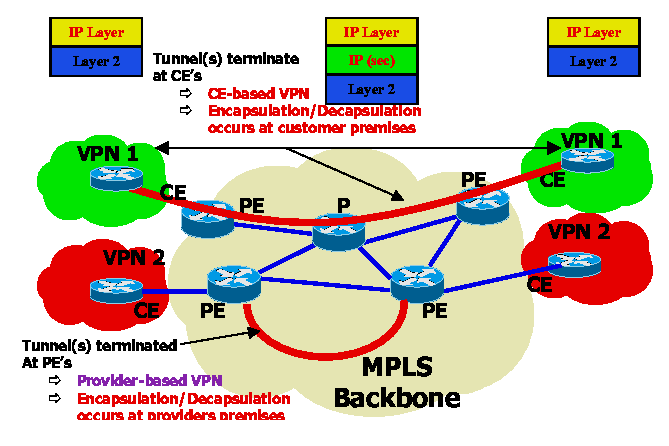
\includegraphics{Figures/CePeVPNs} 
 \caption{Example of CE-based and PE-based VPNs.}
\label{fig:CePeVPNs} 
\end{figure}

CE-based point-to-point VPNs require each router to maintain routing peering with N (CE) devices. This requires the set up of $N\times(N-1)$ connections for full mesh, which will not scale in large networks. With MPLS VPNs, CE only maintains routing peering with one device, which is independent of the total number of sites within the \gls{VPN}.

\subsubsection{PE-based VPNs}
In Provider Edge (PE) based \gls{VPN}, all \gls{VPN} configuration and provisioning are performed on the PE side. The customer edge equipment (CE) connects to the provider PE via a LAN or WAN data link. PE devices hold customer related routes and configurations, while P devices form the backbone devices of the provider�s network. PE-based VPNs solution exists in both Layer-2 and Layer-3. A Layer-3 \gls{VPN} forwards packets based on the \gls{VPN} customer�s packet header IP address. A Layer-2 \gls{VPN}, on the other hand, forwards frames based on information present in the layer 2 frames (e.g. \gls{VLAN}, frames, MAC address, VC Connection Identifiers, etc). Examples of difference PE-based \gls{VPN} implementations are shown in Figure~\ref{fig:CePeVPNs}.

Scalability: only PE routers maintain per-VPN FIBs and run BGP; P routers run IGP only and maintain no VPN state in the core
Customer does not have to maintain virtual backbone, and
the ISP builds/manages tunnels between intra-VPN sites

\subsubsection{Tunnel-based IP VPNs}
In tunnel-based IP-VPNs, a tunnel has two end points where the security service is both negotiated and maintained. Tunneling is a technique used to transfer data for one network over another network. At the start point of the tunnel, the encapsulating protocol adds an outer header over the original packet to form the encapsulated packet. The additional headers provide routing or switching information that enable the encapsulated payload to traverse the intermediate internetwork. At the other end of the tunnel, the outer header is removed and the original packet is recovered. The tunnel itself constitutes the logical path-- otherwise, referred to as a pseudo-wire-- that the encapsulated packets traverse over throughout internetwork.

Tunnels can be applied to various layers in the network protocol stack. It is typically used when transporting or bridging packets belonging to various heterogeneous networks implementing dissimilar protocols for communication. More commonly, tunneling is performed at the data link layer or the network layer.

Tunnels are established across a network for several reasons that include: 

\begin{enumerate}
\item bridging disconnected networks-- for example, to tunnel IPv6 customer packets over an IPv4 \gls{SP} network,
\item providing communication between the home and remote/foreign network in order to reroute traffic destined to the mobile node (\eg in mobile-IP implementation), 
\item providing private and secure communications across a public network,
\item providing connectivity for multiprotocol network layer protocols (\eg System Network Architecture (SNA), IPX, Appletalk, etc.) over a single-protocol backbone, and offering an alternative to source routing.
\end{enumerate}

Tunnels are usually classified based on the type of traffic that they can transport. Example of some Layer-3 IP tunnels include: IP-in-IP (IP/IP), Generalized Routing Encapsulation (GRE), and IPsec tunnels. Layer-2 tunnels include Point-to-Point Tunneling Protocol (PPTP) and Layer 2 Tunneling Protocol (L2TP), and Stacked VLANs (SVLANs). The  Any Transport Over MPLS (AToM) enables MPLS-TE tunnels, however, to
transport Layer-2 as well as Layer-3 traffic. Recently, the IETF has also established a working group named Pseudo Wire Emulation Edge-to-Edge (PWE3) {[}1] which aims at developing standards for the encapsulation
of service-specific PDUs arriving at an ingress logical port and carried across a tunnel.

There are two methods for implementing IP tunnels: 1) the voluntary tunneling and 2) the compulsory tunneling. Voluntary tunneling is client initiated, while compulsory tunneling is initiated at the network access server located at the \gls{ISP}'s point of presence dial-up system. Voluntary tunneling can be used today without requiring any new hardware or negotiating special contracts with an \gls{ISP}.
It is also inherently more scalable than compulsory tunneling, because the tunneling client handles the work of encapsulation and encryption, rather than requiring that this be done on a network device.

\subsection{MPLS-based VPNs}
MPLS offers a scalable IP-VPN solution that delivers value-added services such as security, protection, and support for \gls{QoS} (\eg using \gls{DS-TE}). MPLS also facilitates TE functions by introducing Constraint Shortest Path (\gls{CSPF}) computation features that enable better management of traffic and link utilization in the provider network. Label-Switched Paths (LSPs) can be setup to provide the generic tunneling service to connect segments of a \gls{VPN} over a public provider network, interconnect two non-IP based networks, or define certain treatment (\eg class of service) for packets based on a defined filtering policy. The interior of an MPLS \gls{VPN} network is made up of MPLS-aware P router-devices. PE routers surround the core devices and enable \gls{VPN} functions. P and PE routers act as label switch routers (LSR) that are devices capable of switching packets based on their MPLS-imposed labels.

\subsubsection{Layer-3 MPLS-based VPNs}
The Layer-3 approach to creating MPLS-based VPNs offers a routed solution to the problem. This implementation described in the IETF RFC2547-MPLS/BGP VPNs {[}2] was proposed by the two leader networking solution providers Cisco Systems and Juniper. The approach emphasizes on the use of BGP protocol that already runs at the edges of \gls{ISP} networks and proposes the setup of MPLS LSP-tunnels based on stacked labels that begin and terminate at the PE routers. The inner label identifies the specific \gls{VPN} the packet belongs to, while the outer label determines the path that the packet travels through in the provider network. BGP is used as signaling mechanism for the inner labels while the outer labels� signaling is usually done through LDP or RSVP-TE.

The PE routers exchange routes with the Customer Edge (CE) routers to acquire reachability about the customer's network. These routes are shared with other PE routers carrying the same \gls{VPN}(s) via BGP. Each \gls{VPN} is associated with a \gls{VPN} routing and forwarding instance (VRF). A VRF defines the \gls{VPN} membership of a customer site attached to a PE router. The incoming interface on the PE is used to determine which forwarding table to use when handling a packet because each incoming interface on a PE router is associated with a particular \gls{VPN}. Route Distinguishers (RDs) provide a way of differentiating overlapping routes belonging to different VPNs on the BGP receiver side. When a PE router receives the routes of a given \gls{VPN} site from another PE, it forwards them to the CE router of the connected site belonging to that same \gls{VPN}, so that the CE knows about the networks in the remote site. P routers perform their label switching function without knowledge of the customer's network. Hence, they do not need to share the routes with PE routers.

\subsubsection{Layer-2 MPLS-based VPNs}
The transport of layer-2 traffic, such as Ethernet, Frame Relay or ATM, over an MPLS-enabled transport network has gained recent popularity. Service providers can now use an IP/MPLS core network to offer \gls{VPN}
and Internet access services at the same time. In layer 2 VPNs, the customer data can be forwarded over the MPLS backbone based on information embedded in the layer 2 headers, such as a Frame Relay DLCI, an Ethernet MAC address, or 802.1q \gls{VLAN} tag. Hence, Layer-2 VPNs are inherently Layer-3 protocol transparent, and support the transport of both IP and non-IP traffic. Layer-2 VPNs also eliminate the need
for service providers to participate in a customer�s Layer-3 routing. From a customer�s viewpoint, nothing changes in the network since there are no special requirements on the CE devices and the customer is not exposed to any MPLS technology.

\subsubsection{Layer-2 VLAN-based VPNs}
\gls{VLAN}s represent a standardized Layer-2 mechanism for partitioning a single physical LAN into multiple disjoint logical LANs. \gls{VLAN}s are typically assigned based on the traffic port number, type of the
protocol, the hardware address, or an explicit tag carried within the packet. \gls{VLAN}s provide an efficient mechanism for enhancing performance by reducing the span of a layer 2 broadcast scope. Layer 2 switches isolate traffic across \gls{VLAN} boundaries. Connectivity between distinct \gls{VLAN}s is achieved by routing at layer-3 usually done by a router device. The IEEE 802.1Q standard defines the packet format and required behavior for tagged-based \gls{VLAN}s. The Q tag inserted in the Ethernet frames is limited to 12-bits, or 4096 unique \gls{VLAN} Ids (VIDs). This limits the maximum number of \gls{VLAN}s accommodated within one network.

Stacked VLANs (SVLANs) were introduced to address this shortcoming by adding an additional 4-byte Q-tag header to each tagged packet. SVLANs provide \gls{VLAN} transparency for IEEE 802.1Q tagged or untagged traffic, and can be implemented in a provider network as a PE-based \gls{VPN} solution to provide connectivity to remote \gls{VLAN}s over a publicly share infrastructure. Using this scheme, up to 4096 \gls{VLAN}s can be defined per customer, while the service provider uses up to 4096 SVLANs, increasing the maximum number of accommodated number of \gls{VLAN}s to 4096x4096.

This technology has been widely adapted in Metro Ethernet applications since it provides a very cost effective solution to transport multiple customer \gls{VLAN}s across the service provider's MAN/WAN without interfering with each other. Layer 2 Class of Service (CoS) can further be supported in the core network on per SVLAN basis.

\subsubsection{Layer-1 GMPLS VPNs}
Recently, there has been an increased attention in providing coarse-grained \gls{QoS} using differentiated optical services {[}TOM04]. From the high speed networking perspective, the most promising approach to deliver high bandwidth with the appropriate \gls{QoS} is in an integrated IP over WDM architecture that is facilitated by using the Optical Cross Connect (OXC) and \gls{GMPLS} technologies. The challenge of VPNs in IP/WDM network stems from jointly considering \gls{VPN} provisioning, IP routing, and WDM lightpath configuration. Such a problem can be formulated as a non-linear and non-convex combinatorial optimization problem in which the network construction cost is to be minimized. Problem constraints in this case include \gls{QoS} requirements for \gls{VPN} users and network operators, IP routing
and link capacity assignment, and WDM wavelength configuration constraints.

In IP over WDM network design problem, the two-phase approach is the most common approach. Gouveia et al. {[}GOU03] have proposed a two-phase approach for tackling the MPLS over WDM network design problem. The
first phase solves the core label switching routers placement in MPLS network. The second phase is to determine the physical lightpaths in order to support the logical paths determined in the first phase. However, such an approach sacrifices optimality. Buype et al in {[}PUP03] and {[}PUP05] propose a multi-layer traffic engineering optimization that requires knowledge of the underlying WDM topology. The online
algorithm monitors and reacts to the increase and decrease of bandwidth beyond and below a threshold respectively to set up or tear down links. In our study, we intend to study an integrated approach to jointly
consider the multilayer IP/WDM design problem at the same time, as well take into account VPNs that cross multiple service provider domains.

\begin{figure}
\centering
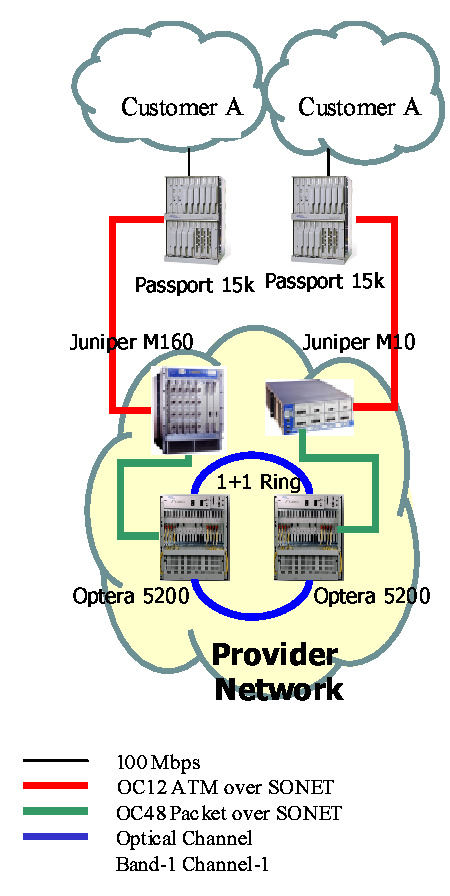
\includegraphics[scale=0.45]{Figures/ProviderNetwork} 
\caption{Layer-3 VPN testbed setup}
\label{fig:ProviderNetwork} 
\end{figure}

\section{Experimental Implementation of Multi-layered VPNs}

In {[}SAA05a] and {[}SAA05c], we published our experiences in the implementation of provider-based VPNs based on different tunneling techniques. Using a metro-based testbed at the Optical Networks Research Lab (ONRL). We described our implementation of several \gls{VPN} tunneling techniques including: 1) Layer-2 virtual circuits using Generic Routing Encapsulation (GRE) {[}HAN94] tunnels, 2) Layer-2 trunks using Ethernet SVLANs {[}IEEE80], 3) Layer-2 tunnels using L2TPv) {[}TOW99], and finally 4) Layer-2 transparent bridging across heterogeneous networks using GRE and L2TPv3 tunnels. Figure~\ref{fig:TBL2VPNs} shows the several configuration setups that were used to implement the mentioned schemes for Layer-2 VPNS.

There are various measurable quantities of interest that can be of indication to the state of the network. For example, available bandwidth, throughput, packet latency, and packet loss, etc. are usually an indication of performance of the network. In this article, we consider the throughput parameter to study different protection schemes that were implemented over the \gls{VPN} solutions discussed earlier.

\begin{figure}
\centering
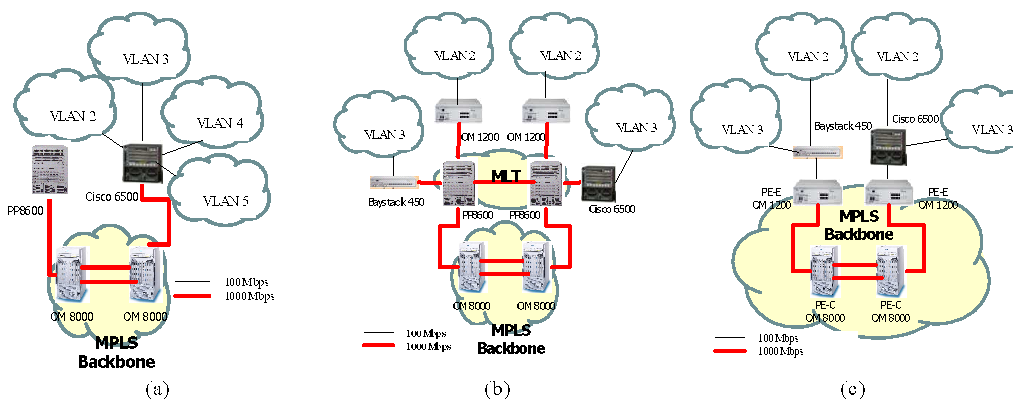
\includegraphics[scale=0.85]{Figures/TBL2VPNs.eps} 
\caption[Layer-2 VPN Testbed setup]
{Layer-2 VPN Testbed setup:
 (a) Switched L2-VPN.
 (b) Transparent L2-VPN.
 (c) VPLS L2-VPN}
\label{fig:TBL2VPNs}
\end{figure}

\subsection{Description of Testbed Hardware}
The testbed that was used to carry out our experiments consisted of multi-vendor equipment from Nortel Networks, Cisco Systems, and Juniper. The Optera Metro 1200 (OM-1200) switch-aggregator was equipped with 10/100 Mbps User to Network Interface (UNI) ports and two Network-to-Network (NNI) Gigabit Ethernet (GigE) interface-cards and were used as CE devices. The Optera Metro 8000 (OM-8000) MPLS switches were equipped with GigE ports and were used in the MPLS backbone. The Passport 8600 (PP-8600) router/switch was equipped with GigE ports and was used as an IP router and as a provider SVLAN-enabled layer 2 switch. The Baystack 425 and Cisco Catalyst 6500 switches were used as an 802.1q-enabled switches that also support layer 2 Class of Service (802.1p) and layer 2 multicast.

Nortel Networks Passport 15K (PP-15K) was used as CE device and was equipped with two OC-12 ATM interfaces, and two FastEthernet ports. Juniper's M-10, and M-160 were used as PE MPLS LSRs, and with OC-48 POS, and OC-12 ATM interfaces. Nortel's OPtera Metro (OM-5200s) DWDM sitches were used as an Optical Add Drop Multiplexer (OADM) for OC-48 POS interfaces. Five Intel-Pentium IV PC-machines were used as traffic sources/sinks in our tests.

Figure 2.5 shows the throughput of TCP flows across the established tunnels described in cases 1 to 4. The throughput was measured while varying the maximum segment size (MSS) of TCP from 350 to 1200 bytes. As expected, as the MSS increased-- \ie\ the payload size increased-- the total number of packets needed to transfer the same amount of data decreased resulting in an increase of the overall throughput of the TCP flow. However, as total packets size exceeded the MTU of the tunnel, we noticed that packets were fragmented before entering the tunnel and defragmented back at the other end point. This resulted in an increase in the overhead and CPU utilization of the routers.

Using a network protocol analyzer, we were able to compute the approximate overhead bytes per packet by sending a 1000-byte UDP datagrams and comparing it with the size of the overall captured packet (after applying tunneling encapsulation in the core of the network). Figure 2.6 shows the overhead per packet as measured when transported over each of the established tunnel in cases mentioned earlier. Results showed that MPLS-based techniques outperformed other IP-based tunneling in terms of overhead in signaling, reliability, scalability and performance. Furthermore, our tests have shown that increasing the size of the transported payload will increase the throughput as long as the packet size does not exceed the MTU size of the established  tunnel. In this case, extra fragmentation and de-fragmentation becomes necessary at the endpoints of the tunnel incurring extra processing power on the routers as well as a decrease in the overall throughput due to the increase in the total overhead.

\begin{figure}
\centering
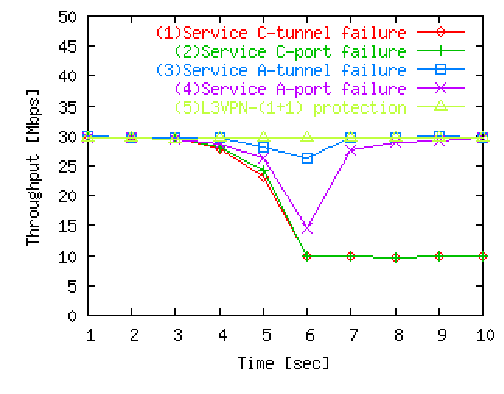
\includegraphics[scale=1]{Figures/ExpResults-01.eps} 
\caption[Throughput of traffic for switched VPN service]%
 {Throughput of traffic for switched VPN service over:
  (1) Service C with tunnel failure,
  (2) Service C with port failure,
  (3) Service A with tunnel failure,
  (4) Service A with port failure, and
  (5) Layer-3 VPN service.}
\label{fig:ExpResults-01}
\end{figure}

\subsection{Experiments Setup}
TODO...


\subsection{Numerical Results}
Figures 6 shows the measured throughput when 30 Mbps of UDP traffic is sent from source-host to a sink-host across the \gls{VPN} implementation scenarios described in previous sections. The abrupt drop in throughput in cases 1 and 2 (at approximately t= 6 secs) coincides with the time that the fault was injected on the primary connection. As expected, recovery from the failure was faster in the case of tunnel failure in one direction as opposed to port failure that brings down the tunnels in both directions of the primary connection. On the other hand, service C (which resembles a best-effort service in our test setup) was allowed only the available bandwidth on the backup tunnels (10 Mbps in this case) -- only after service A had been assigned its full backup capacity. Case 5 shown in Figure 5 represents the throughput of the same UDP traffic transferred over layer-3 \gls{VPN} implementation scenario. In this case, we estimated recovery time of the \gls{VPN} connection between the 2 OM-8000s to be around 27 msec. The downgrade in throughput was barely noticeable.


\section{Evaluation of Protocol Overhead for Tunnel Techniques}
In this experiment, we try to compare the performance characteristics of various tunneling implementations and their impact on the end-to-end data throughput. In each case, an end-to-end virtual connection is established using a tunnel or a series of concatenated tunnels spanning different heterogeneous provider domains each implementing a different tunneling technique. The concatenated tunnels constitute a virtual connection that interconnects remote customer \gls{VLAN} sites.

Generally, there are two types of inter-provider relations that co-exist between different network operators, namely: the peer-to-peer model, and the client-server model. In the client-server model the client domain requests service that the server domain offers. Client network domains receive transport services from their service provider to reach each other. In the peer model, a client network domain is treated as a peer of its service-provider; hence, peer domains not only receive transport services from other participating domains but also contribute new transport services to other domains. For our tests, the Iperf tool was used to generate traffic and measure throughput. Iperf is a tool capable of measuring a number of parameters including bandwidth, throughput, delay jitter, and packet loss.

\subsection{Description of Testbed Hardware}
The testbed that was used to carry out our experiments consisted of equipment from Nortel Networks, Cisco Systems, Juniper and Navtel. The Nortel Optera Metro 8000s (OM-8000s) MPLS switches were equipped with Gigabit Ethernet (GigE) ports, and were used in the ONRL-L2 MPLS domain. The Passport 8600s (PP-8600s) router/switches were equipped with GigE ports and were used in the ONRL-SVLAN domain. The Cisco 3745 routers were equipped with GigE ports and Fast Ethernet (FE) ports, and were used in the IP-based CRC-domain. The Juniper M-10 and M-160 were equipped with GigE ports and OC-12 ATM over SONET interfaces, and were used as Prvider Edge (PE) routers in the ONRL-L3 MPLS based network. Two Intel-based Pentium IV machines equipped with a GigE port were placed in each of the customer�s remote \gls{VLAN}-sites, and were used as traffic sources/sinks in our tests. The Navtel protocol analyzer was used to capture test traffic in order to measure the overall performance and tunnel overhead.

\begin{figure}
\centering
\subfloat[Normalized TCP flow throughput for the implemented tunnel scenario versus maximum segment size.]
{\label{fig:MssThruput}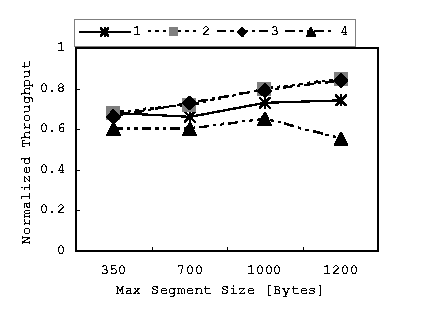
\includegraphics{Figures/MssThruput.eps}}
\quad
\subfloat[Percentage of maximum packet overhead per packet for established tunnels for a 1000-byte packet.]
{\label{fig:TunOverhead}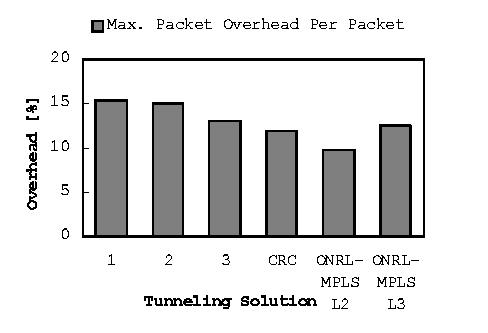
\includegraphics{Figures/TunOverhead.eps}}
\caption{Experimental results}
\label{fig:OverheadResults} 
\end{figure}

\subsection{Experiments Setup}
The purpose of the experiments is to transport \gls{VLAN} traffic over networks running heterogeneous transport protocols. 1) Implementing L2 virtual circuit using GRE: In this setup, the CRC IP-domain, and the ONRL-L2 MPLS domains are employed. The ONR-L2 runs MPLS tunneling service to provide transparent transport for Ethernet VLAN-tagged traffic between the two end PC-clients in the remote \gls{VLAN}s as shown in Fig. 3. In this case, the CRC domain is totally contained inside the ONRL-L2 domain and runs Ethernet over IP-based GRE tunneling service in order to stitch LSPs crossing it from side to side. Ethernet encapsulated MPLS packets arriving at one of the CRC border routers are encapsulated within IP/GRE packets, and then forwarded towards the other border router where it gets decapsulated back to an MPLS over Ethernet datagram and forwarded to the neighboring LSR. Fig. 3 shows the packet encapsulation at each of the mentioned stages.

2)Implementing L2 trunking using S-VLANs: For this experiment, the ONRL-SVLAN and the ONRL-L2 MPLS domains are configured to provide a tunnel connection for the remote PC-clients present in the customer \gls{VLAN}s as shown in Fig. 4. The ONRL-L2 provides transparent transport for Ethernet \gls{VLAN}-tagged traffic over MPLS L2 tunnels. The ONRL-SVLAN domain is totally contained inside ONRL-L2 domain and runs SVLAN tunneling service in order to stitch LSPs crossing its domain boundaries. The Ethernet encapsulated MPLS packets arriving at one of the ONRL-SVLAN border-routers are wrapped within SVLAN packets and forwarded towards the next border router where they are decapsulated back to MPLS over Ethernet frames and forwarded to the neighboring LSR. Fig. 4 shows the Packet encapsulation at each of the mentioned stages. 3) Implementing Ethernet transparent bridging using L2TPv3 tunnels: In this setup, the CRC IP domain and the ONRL-L2 MPLS domains are configured to provide the same service for the PC clients in the customer \gls{VLAN}s as shown in Fig. 3. The CRC domain uses L2TPv3 to establish tunnels that carry VLAN-tagged Ethernet frames encapsulated over MPLS. The Packet encapsulation at each of the mentioned stages is shown in Fig. 3.

4) Implementing Ethernet transparent bridging across heterogeneous network: In this experiment, the CRC, ONRL-L2 and ONRL-L3 are arranged as peer domains that provide transit tunneling-service to end-to-end connections between the PCs in the customer VLAN networks. The ONRL-L2 MPLS and CRC IP domains are configured to provide the same services as described in experiment 1 and 2. The ONRL-L3 domain is configured to provide a layer-3 tunneling service over MPLS as per RFC-2547bis. In order to transfer layer-2 VLAN-tagged frames over layer-3 MPLS tunnels, an IP/GRE tunnel is first established between the ONRL-L3 edge routers. The VLAN-tagged frames are first encapsulated over IP/GRE and then encapsulated over MPLS packets. At the egress edge router, the MPLS and IP/GRE headers are extracted and the VLAN-tagged frame is restored back and forwarded to the customer network as shown in Fig. 5.


\subsection{Numerical Results}
Figure~\ref{fig:MssThruput} shows the throughput of the TCP flow across the established tunnels described in cases 1 to 4. The throughput was measured while varying the maximum segment size MSS) of TCP from 350 to 1200 bytes. As expected, as MSS increased- i.e the payload size increased- the total number of packets needed to transfer the same amount of data decreased resulting in an increase of the overall throughput of the TCP flow. However, as total packets size exceeded the MTU of the tunnel, we noticed that packets were fragmented before entering the tunnel and defragmented back at the other end point. This resulted in an increase in the overhead and CPU utilization of the routers. Figure~\ref{fig:TunOverhead} shows the overhead per packet measured when transported over each of the established tunnel in cases mentioned earlier. In cases 1 and 3, the maximum overhead occurred across the CRC domain. In this case the overhead was composed of an IP, Ethernet VLAN, MPLS, Ethernet, GRE/L2TPv3, IP, and Ethernet header. For case 2, the maximum overhead occurred across the ONRL-SVLAN domain and was composed of an IP, ethernet vlan, mpls, Ethernet, SVLAN header. In case 4, Fig. 7 shows the overhead in each of the three domains: ONRL-L2, CRC and ONRL-L3 individually. In the ONRL-L3 domain, the overhead was composed of an IP, Ethernet VLAN, GRE, IP, MPLS, and Ethernet header.

\section{Conculsions}
In this chapter, we gave an overview of the architectural structure of existing hierarchical transport networks and its different abstraction layers. We highlighted the challenges posed in performing multi-layer traffic engineering and \gls{QoS} routing across vertical and horizontal layers for hierarchical networks. Three basic models for the control plane implementation in \gls{GMPLS} networks were also considered, namely: overlay, full-peer, and border model. The border model is seen as a promising architectural model that addresses the full-peer model�s scalability problems � by only exchanging partial information between switching layers� and offers better utilization than the overlay model by introducing new intelligent PCE schemes at border or edge nodes that can base their path computation based on information from multiple layers. In our work, we will propose to utilize the border model architecture, while revising and extending the information exchanged by \gls{GMPLS} border routers for different domains or switching layers.

This chapter also introduced multilayered VPNs, including traditional layer-3, layer-2, and layer-1 optical VPNs. We presented our findings in some of the works that we have concluded in this area. In Chapter 3, we will consider the survivability issues in multilayered transport networks.
